\documentclass[12pt,a4paper]{article}
\usepackage[utf8]{inputenc}
\usepackage[spanish]{babel}
\usepackage{amsmath}
\usepackage{amsfonts}
\usepackage{amssymb}
\usepackage{graphicx}
\usepackage{kpfonts}
\usepackage[left=2cm,right=2cm,top=2cm,bottom=2cm]{geometry}
\title{EV 2-3 ARREGLOS Y PARÁMETROS EN AMPLIFICADORES CLASE B

\includegraphics [scale=1]{imagenes/UPZMG.png} 
\author{Giovanni Daniel Ruiz Tinoco\\
\small Sistemas electrónicos de interfaz\\
  \small Universidad Politécnica de la zona metropolitana de Guadalajara\\
  \small 4°B \\
  \small Ing. Mecatrónica\\
\centering
\linebreak
}
}

\begin{document}
\maketitle
\newpage
\begin{flushleft}
\section {cuales son los los amplificadores clase B?}
\end{flushleft}
Se les denomina amplificador clase B, cuando el voltaje de polarización y la máxima amplitud de la señal entrante poseen valores que hacen que la corriente de salida circule durante el semiciclo de la señal de entrada.

La característica principal de este tipo de amplificadores es el alto factor de amplificación. 

Los amplificadores de Clase B usan dos o más transistores polarizados de tal forma que cada transistor solo conduce durante un medio ciclo de la onda de entrada, Para mejorar la eficiencia de potencia total del amplificador de clase A previo reduciendo la potencia desperdiciada en forma de calor, es posible diseñar el circuito amplificador de potencia con dos transistores en su etapa de salida produciendo lo que comúnmente se denomina amplificador de clase B también. conocido como una configuración de amplificador push-pull .
\begin{center}
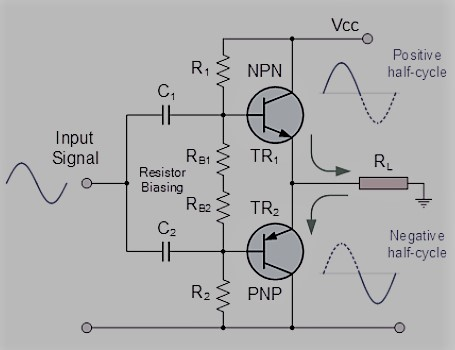
\includegraphics[scale=.8]{imagenes/amplificadorB.JPG} 
\end{center}
\begin{flushleft}
\subsection{Ventajas}
-Es de bajo consumo en reposo
\linebreak
-Aprovecha al máximo la corriente de la fuente
\linebreak
-Intensidad casi nula en reposo (poca generación de calor)
\subsection{desventajas}
-Producen armónicos, y es mayor cuando no tienen los transistores de salida con las mismas características técnicas, debido a esto se les suele polarizar de forma que se les introduce una pequeña polarización directa. Con esto se consigue desplazar las curvas y se disminuye dicha distorsión.
\linebreak
\linebreak
\end{flushleft}
\begin{flushleft}
\section {Arreglos en amplificadores clase B}
Los amplificadores Push-Pull utilizan dos transistores "complementarios" o coincidentes, uno de tipo NPN y el otro de tipo PNP con ambos transistores de potencia que reciben la misma señal de entrada que es igual en magnitud, pero en fase opuesta entre sí . Esto resulta en un transistor solamente amplificar la mitad o 180 o del ciclo de forma de onda de entrada mientras que el otro transistor amplifica la otra mitad o restante 180 o del ciclo de forma de onda de entrada con las resultantes de “dos mitades” está poniendo juntos de nuevo en la salida terminal.

A continuación, el ángulo de conducción para este tipo de circuito amplificador sólo es 180 o 50 por ciento de la señal de entrada. Este efecto de empujar y tirar de los semiciclos alternos por los transistores da a este tipo de circuito su divertido nombre push-pull, pero en general se lo conoce como el amplificador de clase B, como se muestra a continuación.
\linebreak
\end{flushleft}
\subsection{Circuito Amplificador de Transformador Push-pull de Clase B}
\begin{center}
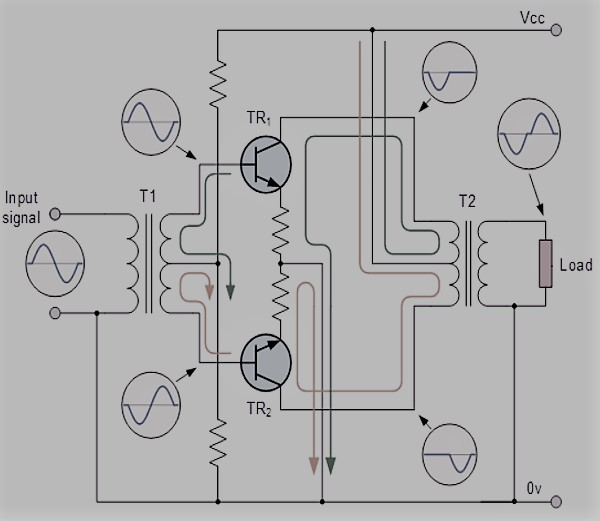
\includegraphics[scale=.5]{imagenes/1ETAPA.JPG} 
\end{center}
\begin{flushleft}
El circuito anterior muestra un circuito amplificador Clase B estándar que utiliza un transformador de entrada con toma central compensada, que divide la señal de forma de onda entrante en dos mitades iguales y que están desfasadas 180 ° entre sí. Otro transformador con toma central en la salida se utiliza para recombinar las dos señales que proporcionan la mayor potencia a la carga. Los transistores utilizados para este tipo de circuito amplificador push-pull de transformador son ambos transistores NPN con sus terminales de emisor conectados entre sí.\linebreak

Aquí, la corriente de carga se comparte entre los dos dispositivos de transistor de potencia a medida que disminuye en un dispositivo y aumenta en el otro a lo largo del ciclo de señal, reduciendo el voltaje y la corriente de salida a cero. El resultado es que ambas mitades de la forma de onda de salida ahora oscilan desde cero hasta el doble de la corriente de reposo, reduciendo así la disipación. Esto tiene el efecto de casi duplicar la eficiencia del amplificador a alrededor del 70.\linebreak

Suponiendo que no haya señal de entrada presente, entonces cada transistor lleva la corriente de colector quiescente normal, cuyo valor está determinado por la polarización de la base que está en el punto de corte. Si el transformador está centrado exactamente, las dos corrientes del colector fluirán en direcciones opuestas (condición ideal) y no habrá magnetización del núcleo del transformador, lo que minimiza la posibilidad de distorsión.\linebreak

Cuando una señal de entrada está presente en el secundario del transformador controlador T1 , las entradas de la base del transistor están "antifásicas" entre sí como se muestra, por lo tanto, si la base TR1 es positiva y conduce el transistor a conducción pesada, su corriente de colector aumentará pero al mismo tiempo, la corriente de base de TR2 se volverá negativa en el corte y la corriente de colector de este transistor disminuirá en una cantidad igual y viceversa. Por lo tanto, las mitades negativas son amplificadas por un transistor y las mitades positivas por el otro transistor dando este efecto de contrafase.
\linebreak
\end{flushleft}
\begin{flushleft}
\subsection{Curvas de características de salida de clase B}
El amplificador de clase B tiene la gran ventaja sobre sus primos de amplificador de clase A en que ninguna corriente fluye a través de los transistores cuando están en estado de reposo (es decir, sin señal de entrada), por lo tanto no se disipa potencia en los transistores de salida o transformador cuando no hay señal presente a diferencia de las etapas de amplificador de Clase A que requieren un sesgo de base significativo, disipando así gran cantidad de calor, incluso sin presencia de señal de entrada.
\linebreak
\linebreak
Por lo tanto, la eficiencia total de conversión del amplificador es mayor que la de la Clase A equivalente, alcanzando eficiencias tan altas como 70 por ciento, lo que resulta en casi todos los tipos modernos de amplificadores push-pull operados en este modo Clase B.
\linebreak
\linebreak
\end{flushleft}
\begin{center}
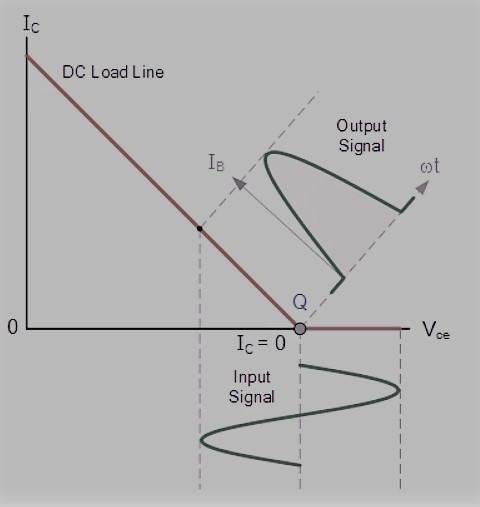
\includegraphics[scale=.6]{imagenes/transformador.JPG}
\end{center}
\newpage 
\section{Amplificador de empuje y tracción de clase B sin transformador}
\begin{flushleft}
Una de las principales desventajas del circuito amplificador Clase B anterior es que utiliza transformadores de derivación central equilibrada en su diseño, por lo que es costoso de construir. Sin embargo, hay otro tipo de amplificador de Clase B llamado Amplificador de Clase B de Simetría Complementaria que no usa transformadores en su diseño, por lo tanto, es sin transformador usando pares de transistores de potencia complementarios o coincidentes.\linebreak

Como los transformadores no son necesarios, esto hace que el circuito del amplificador sea mucho más pequeño para la misma cantidad de salida, también no hay efectos magnéticos extraños o distorsión del transformador para afectar la calidad de la señal de salida. A continuación, se proporciona un ejemplo de un circuito amplificador Clase B "sin transformador".\linebreak
\begin{flushleft}
\subsection{Etapa de salida sin transformador clase B}
\begin{center}
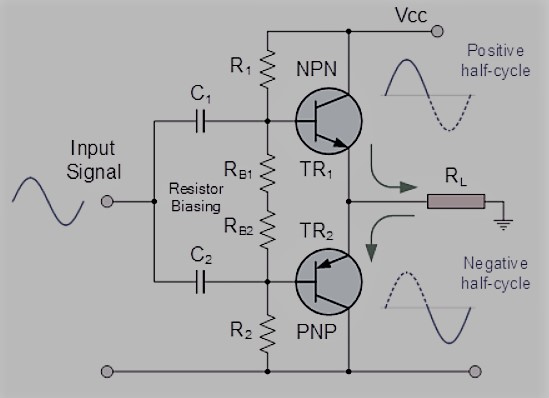
\includegraphics[scale=0.6]{imagenes/parametros.JPG} \linebreak
\end{center}
El circuito amplificador de Clase B anterior usa transistores complementarios para cada mitad de la forma de onda y mientras que los amplificadores de Clase B tienen una ganancia mucho mayor que los tipos de Clase A, una de las principales desventajas de los amplificadores de tipo push-pull de clase B es que sufren una efecto conocido comúnmente como distorsión cruzada .\linebreak

Esperamos recordar de nuestros tutoriales sobre transistores que se necesitan aproximadamente 0,7 voltios (medidos desde la base hasta el emisor) para obtener un transistor bipolar para comenzar a conducir. En un amplificador de clase B puro, los transistores de salida no están "predispuestos" a un estado de funcionamiento encendido.\linebreak

Esto significa que la parte de la forma de onda de salida que cae por debajo de esta ventana de 0.7 voltios no se reproducirá con precisión como la transición entre los dos transistores (cuando cambian de un transistor a otro), los transistores no se detienen o comienzan a conducir exactamente en el punto de cruce cero, incluso si son pares especialmente coincidentes.\linebreak

Los transistores de salida para cada mitad de la forma de onda (positiva y negativa) tendrán cada uno un área de 0,7 voltios en la que no están conduciendo. El resultado es que ambos transistores se apagan al mismo tiempo.\linebreak
\section{El amplificador clase AB}
\begin{center}
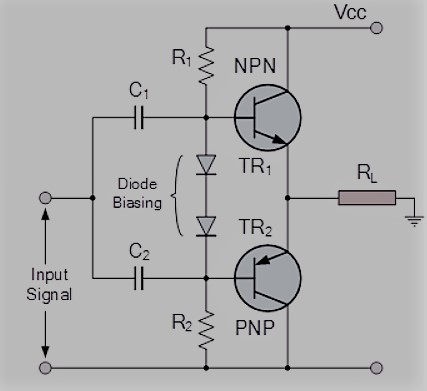
\includegraphics[scale=0.6]{imagenes/AB.JPG}
\end{center}
El circuito amplificador Clase AB es un compromiso entre las configuraciones Clase A y Clase B. Este voltaje de polarización de diodo muy pequeño hace que ambos transistores conduzcan ligeramente incluso cuando no hay señal de entrada presente. Una forma de onda de la señal de entrada hará que los transistores funcionen normalmente en su región activa, eliminando así cualquier distorsión de cruce presente en los diseños puros de la Clase B.\linebreak

Una pequeña corriente de colector fluirá cuando no haya señal de entrada pero es mucho menos que eso para la configuración del amplificador de Clase A. Esto significa entonces que el transistor será ON para más de la mitad de un ciclo de la forma de onda pero mucho menos que un ciclo completo que da un ángulo de conducción de entre 180 o a 360 o o 50 a 100 por ciento de la señal de entrada dependiendo de la cantidad de sesgo adicional utilizado. La cantidad de voltaje de polarización del diodo presente en el terminal base del transistor se puede aumentar en múltiplos mediante la adición de diodos adicionales en serie.\linebreak

Los amplificadores de clase B son muy preferidos sobre los diseños de clase A para aplicaciones de alta potencia como amplificadores de potencia de audio y sistemas de PA. Al igual que el circuito amplificador de clase A, una forma de aumentar en gran medida la ganancia de corriente ( A*i ) de un amplificador push-pull de Clase B es utilizar pares de transistores Darlington en lugar de transistores únicos en su circuito de salida.\linebreak

\section{Referencias bibliográficas}
\begin{flushleft}
Luis González . (2016). Amplificadores Clase B – Generalidades. 09/10/19, de unicrom Sitio web: https://unicrom.com/amplificadores-clase-b-generalidades/ \linebreak


Arturo R. (2014). Amplificador de clase B y amplificador de transistor de clase B . 09/10/19, de blogger Sitio web: http://tutorialesdeelectronicabasica.blogspot.com/2018/06/amplificador-de-clase-b-y-amplificador.html \linebreak

Anonimo. (2012). Amplificador Clase B. 09/10/19, de Ecured Sitio web: https://www.ecured.cu/AmplificadorClaseB

\end{flushleft}
\end{flushleft}
\end{flushleft}
\end{document}

\section{se}